%        File: homework2.tex
%     Created: Fri Jan 23 01:00 PM 2015 P
% Last Change: Fri Jan 23 01:00 PM 2015 P
%
\documentclass[11pt]{article}
\usepackage{geometry}
\usepackage{graphicx}
\geometry{letterpaper}
\usepackage[parfill]{parskip}
\title{Math 360 Homework 2}
\author{Alex Schneider}
\begin{document}
\maketitle
\section*{Handout}
\subsection*{Problem 1}
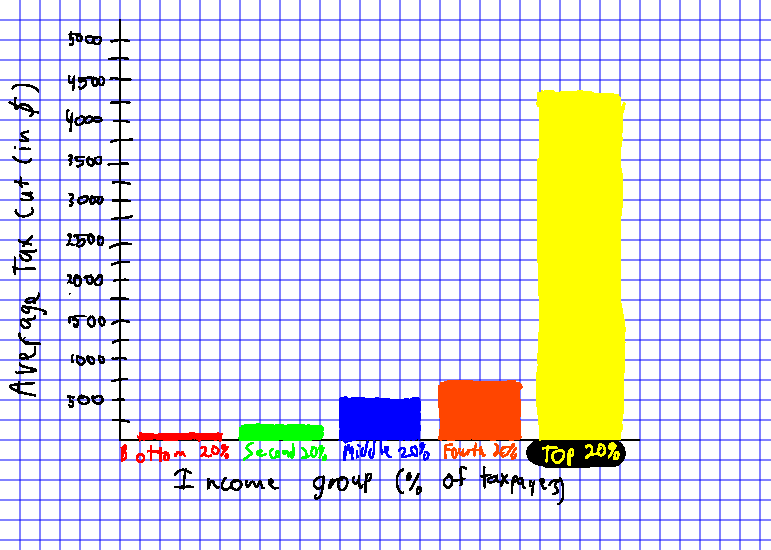
\includegraphics{homework2_handout_problem1_bargraph}

\subsection*{Problem 2}
Given the three values of \$0, \$289, and \$1211, and being asked to determine which
ones are the mean, median, and mode of the tax cuts, I would probably come up
with the following conclusions:

\subsubsection*{Mode}
\[M_0 = \$0\]
Due to the nature of money, nice round numbers out of these types of tax cuts
rarely happen. Therefore, the only round number that we can reasonably expect
is no tax cuts at all, and even if there a relatively few number of people who
received that, it is still a more likely outcome. 

Secondly, it is unlikely for the median or mean to be 0, unless tax cuts are
negative, which they don't appear too be. 

\subsubsection*{Median}
\[M_d = \$289\]
We established that the median cannot be 0. We also know that the median has to 
be somewhere between the second 20\% (\$212) and fourth 20\% (\$951). This
prevents \$1211 from being the median, so we're left with \$289 as our only
option.

\subsubsection*{Mean}
\[\overline{X} = \$1211\]
By process of elimination, we're left with \$1211 as the only candidate for the
mean. In addition, we know that there are a large amount of outliers in the top
20\% which can bring the mean up pretty drastically.

\subsection*{Problem 3}
If I could draw a new bar graph reflecting the new information, I would reach
the limits of information provided by a linear scale. The outliers are so high
that the bar graph would either need to be incredibly large or there would need
to be a misleading break in the middle of the graph. If that were the case, I
would probably go for a graph on a \textit{log} scale to give a more faithful
representation to the data, at the cost of misleading those unfamiliar with
logarithms into thinking the difference is much less than it is. 

\section*{Section 1.3}
\subsection*{Problem 1}
\subsubsection*{a.}
\begin{tabular}{r|l} % chktex 44
    Stem & Leaf \\
    \hline % chktex 44
    0 & 011112235677 \\
    1 & 235579 \\
    2 & 468 \\
    3 & 11257 \\
    4 & 1469 \\
    5 & 5 \\
    6 & 16 \\
    7 & 9 \\
    8 & 0099 \\
    11 & 0 \\
    12 & 7 \\
    13 & 7
\end{tabular}

\subsubsection*{b.}
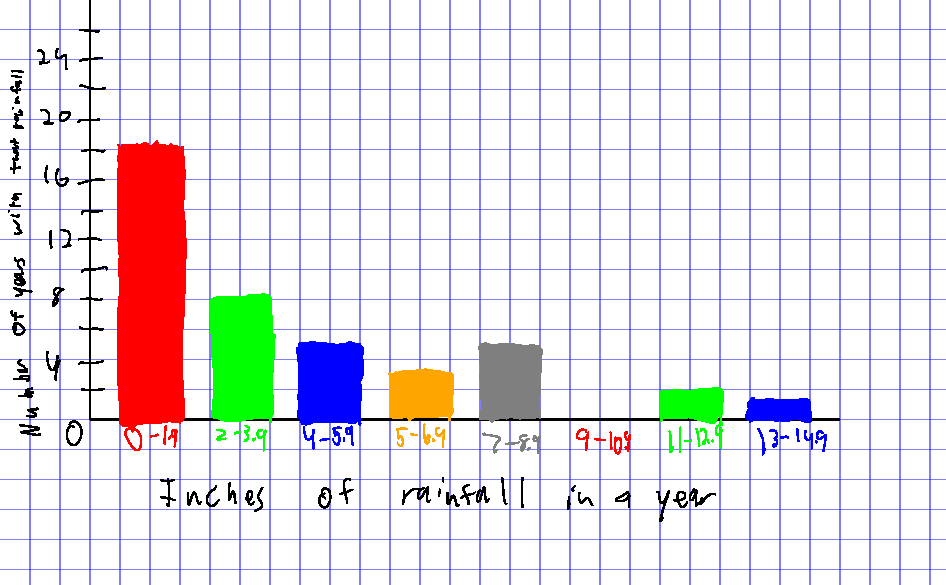
\includegraphics{homework2_section13_problem1b_histogram}

\subsubsection*{c.}
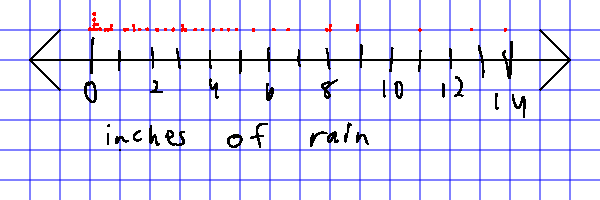
\includegraphics{homework2_section13_problem1c_dotplot}

\subsubsection*{d.}
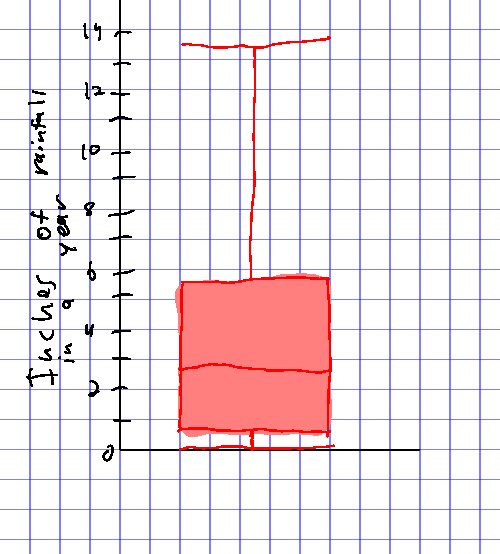
\includegraphics{homework2_section13_problem1d_boxandwhisker}

Yes, the box plot appears to show significant outliers at the top of the
rainfall measurements. 

\subsection*{Problem 2}
\subsubsection*{b.}
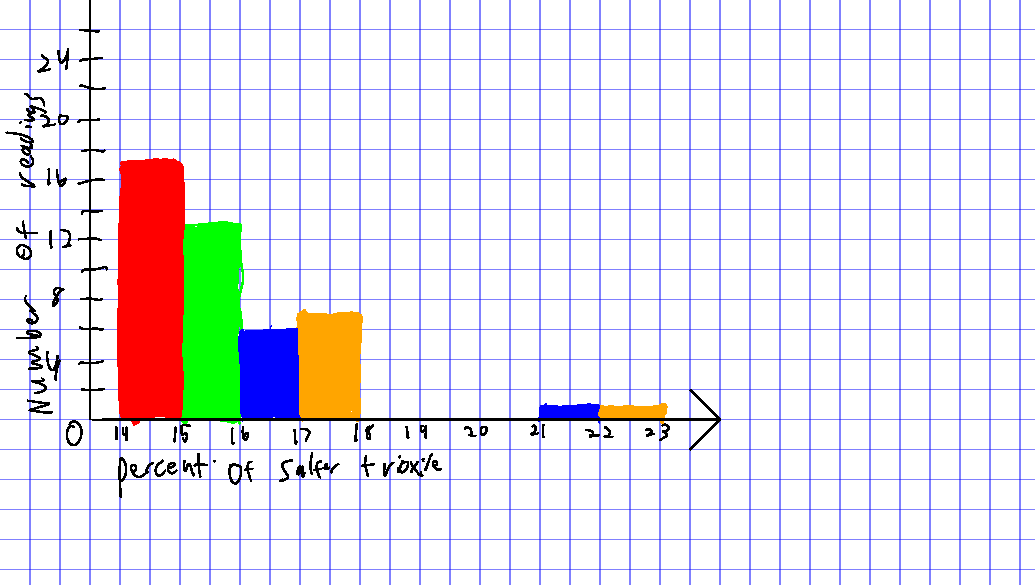
\includegraphics{homework2_section13_problem2b_histogram}

\subsubsection*{c.}
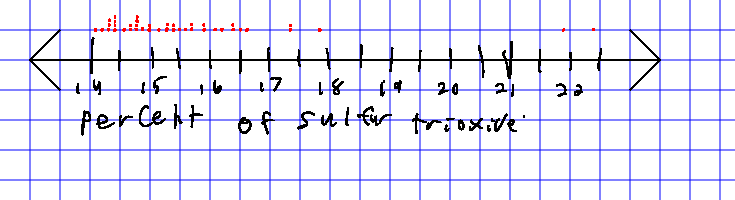
\includegraphics{homework2_section13_problem2c_dotplot}

\subsection*{Problem 6}
\subsubsection*{a.}
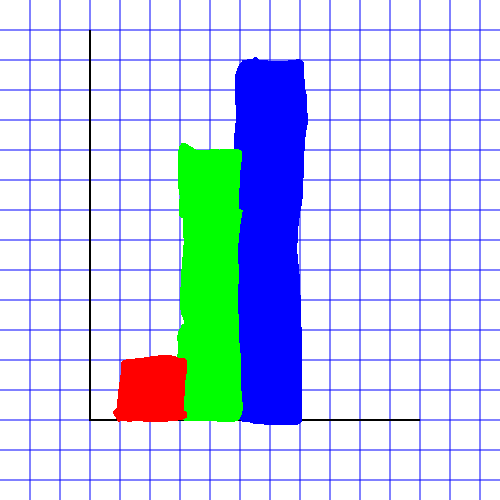
\includegraphics{homework2_section13_problem6a_histogram}

\subsubsection*{b.}
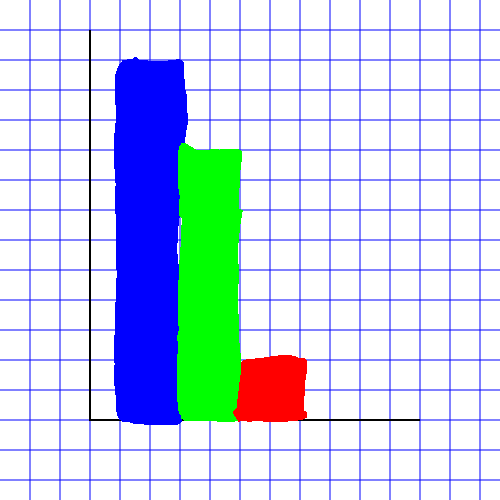
\includegraphics{homework2_section13_problem6b_histogram}

\subsubsection*{c.}
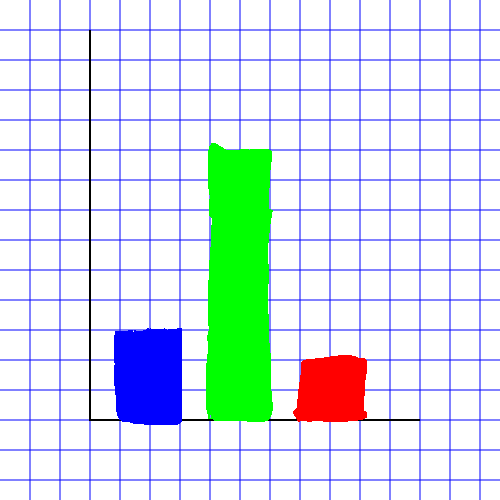
\includegraphics{homework2_section13_problem6c_histogram}

\subsection*{Problem 7}
\subsubsection*{a.}
The percentage of women with blood pressures above 130mm is likely closest to
25\% of the sample represented by the histogram. 

\subsubsection*{b.}
There are more women in the 130--135mm interval.

\subsection*{Problem 12}

\subsection*{Problem 16}

\subsection*{Problem 18}

\section*{Section 2.1}
\subsection*{Problem 1}

\subsection*{Problem 2}

\subsection*{Problem 3}

\subsection*{Problem 4}

\subsection*{Problem 7}

\subsection*{Problem 8}

\subsection*{Problem 9}

\subsection*{Problem 12}

\subsection*{Problem 13}

\subsection*{Problem 17}

\subsection*{Problem 18}

\subsection*{Problem 19}

\end{document}


